\documentclass[11pt,aspectratio=43,ignorenonframetext,t]{beamer}
% Uses fontspec - assumes compiled with LuaLaTeX or similar
% The above \documentclass is for making slides. If making handouts use:
%\documentclass[11pt,a4paper]{article} 
%\usepackage{beamerarticle}
%\setjobnamebeamerversion{main.beamer}

% See https://github.com/CASSON-LAB/uom_beamer_template
% for details on license, further useage information and similar
%%%%%%%%%%%%%%%%%% DOCUMENT SETUP %%%%%%%%%%%%%%%%%%

% Presentation settings
\mode<presentation>{
  \usetheme[framenumber,titleframestart=1]{UoM_alex}
  \usefonttheme{professionalfonts} % using non standard fonts for beamer
  \usefonttheme{serif}             % set font to Arial
  \usepackage{fontspec}
  \setmainfont[Ligatures=TeX]{Arial}
}

% Handout settings
\mode<article>{
  \usepackage{fullpage}                  % use full page
  \usepackage{fontspec}                  % set font to Arial
    \setmainfont[Ligatures=TeX]{Arial}
  \setlength{\parskip}{1.5\baselineskip} % correct beamer line spacings
  \setlength{\parindent}{0cm}
  \usepackage{enumitem}
    \setlist[itemize]{topsep=0pt}
  \definecolor{uomlinkblue}{HTML}{0071BC}
}


% Packages

% Configurando layout para mostrar codigos C++
\usepackage{listings}
\lstset{
  language=HTML,
  basicstyle=\ttfamily\small, 
  keywordstyle=\color{blue}, 
  stringstyle=\color{red}, 
  commentstyle=\color{red}, 
  extendedchars=true, 
  showspaces=false, 
  showstringspaces=false, 
  numbers=left,
  numberstyle=\tiny,
  breaklines=true, 
  backgroundcolor=\color{green!10},
  breakautoindent=true, 
  captionpos=b,
  xleftmargin=0pt,
}

\usepackage{graphicx}  % for graphics files
  \graphicspath{ {./fig/aula2} }
\usepackage{amsmath}   % assumes amsmath package installed
  \allowdisplaybreaks[1] % allow eqnarrays to break across pages
\usepackage{amssymb}   % assumes amsmath package installed 
\usepackage{hyperref} % add hyperlinks to document. Settings are for accessiblity
  \hypersetup{
    colorlinks=true,
    linkcolor=uomlinkblue,
    filecolor=uomlinkblue,      
    urlcolor=uomlinkblue,
	pdflang={en-GB},
}
\usepackage[document]{ragged2e} % left aligned text for accessibility
% experimental - does fundamentally work, if with quite a bit of effort
%\usepackage{axessibility} % LaTeX readable equations for accessibility
%  \tagpdfsetup{tabsorder=structure,uncompress,activate-all,interwordspace=true}
%  \pdfextension catalog{/Lang (en-GB)}
%  \RequirePackage{luacode}
%  \directlua{require("axessibility.lua")}
\usepackage{unicode-math} % unicode maths for accessibility
\usepackage{pdfcomment} % for alt text for accessibility
\usepackage{rotating}  % allow portrait figures and tables
\usepackage{subfigure} % allow matrices of figures
\usepackage{float}     % allows H option on floats to force here placement
\usepackage{multirow}  % allows merging of rows in tables
\usepackage{tabularx}  % allows fixed width tables
\usepackage{ctable}    % modifies \hline for use in table
\usepackage{bm}        % allow bold fonts in equations
\usepackage{pgf}       % allow graphics manipulation
\usepackage{media9}    % allow interactive flash files to be embedded
  \addmediapath{../media}
\usepackage{etoolbox}
  \makeatletter \preto{\@verbatim}{\topsep=0pt \partopsep=0pt} \makeatother  
  
% Custom commands
\newcommand{\matlab}{\emph{\sc{Matlab}}}
\newcommand{\maple}{\emph{\sc{Maple}}}
\newcommand{\simulink}{\emph{\sc{Simulink}}}
\newcommand{\dc}{d.c.}
\newcommand{\ac}{a.c.}
\newcommand{\rms}{RMS}
\newcommand{\wgn}{{\tt wgn}}
\newcommand{\sus}[1]{$^{\mbox{\scriptsize #1}}$}
\newcommand{\sub}[1]{$_{\mbox{\scriptsize #1}}$}
\newcommand{\chap}[1]{Chapter~\ref{#1}}
\newcommand{\sect}[1]{Section~\ref{#1}}
\newcommand{\fig}[1]{Fig.~\ref{#1}}
\newcommand{\tab}[1]{Table~\ref{#1}}
\newcommand{\equ}[1]{(\ref{#1})}
\newcommand{\appx}[1]{Appendix~\ref{#1}}
\newcommand{\degree}{\ensuremath{^\circ}}
\newcommand{\Vrms}{Vrms}
\newcommand{\Vpp}{V\sub{pp}}
\newcommand{\otoprule}{\midrule[\heavyrulewidth]}         
\newcolumntype{Z}{>{\centering\arraybackslash}X}  % tabularx centered columns 
\makeatletter \DeclareRobustCommand{\em}{\@nomath\em \if b\expandafter\@car\f@series\@nil \normalfont \else \bfseries \fi} \makeatother
\newcounter{example_number} % keep track of the example questions



%%%%%%%%%%%%%%%%%% FRONT MATTER %%%%%%%%%%%%%%%%%%
\title{Análise Orientada a objetos}
\subtitle{Aula 2}
\author{Prof. Me. Juliana Costa-Silva}
\begin{document}
%%%%%%%%%%%%%%%%%% TITLE SLIDE %%%%%%%%%%%%%%%%%%
\mode<presentation>{ \frame{\titlepage \label{slide:a}}} 
%\begin{figure}[!ht] 
%\fbox{\includeslide[width=\textwidth]{slide:a}} \end{figure}



%%%%%%%%%%%%%%%%%% NEW SLIDE %%%%%%%%%%%%%%%%%%
\clearpage 
\mode<presentation>{ \begin{frame}{Na aula de hoje...}
  \setbeamertemplate{section in toc}[sections numbered]
  \tableofcontents[hideallsubsections]
\end{frame}}
%-----------------------------------------------------------------------
\section{Strings}
\mode<presentation>{ \begin{frame}{Concatenação de String} 
A concatenação de String é realizada com o uso do operador (+)
\begin{block}{Sintaxe:}
 $<$String1$>$ + $<$String2$>$ = $<$String1String2$>$\\
 \vspace{0.5cm}
 
 $<$String$>$ + $<$DadoPrimitivo$>$ = $<$StringDadoPrimitivo$>$\\
\end{block}

\end{frame}}
%----------------------------------------------------------------
\mode<presentation>{ \begin{frame}{Exemplo Concatenação}
  \begin{center}
   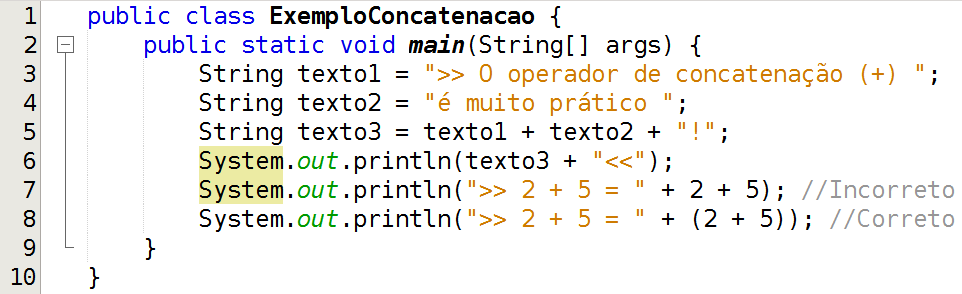
\includegraphics[height=0.37\paperheight]{exemploConcatenacao.png} \\
   
   \textbf{Saída}\\
   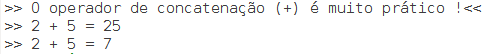
\includegraphics[height=0.1\paperheight]{exemploConcatencaoOut.png} \\
 \end{center}
\end{frame}}
%-------------------------------------
\section{Caracteres Especiais}
\mode<presentation>{ \begin{frame}{Caracteres especiais}
\begin{center}
   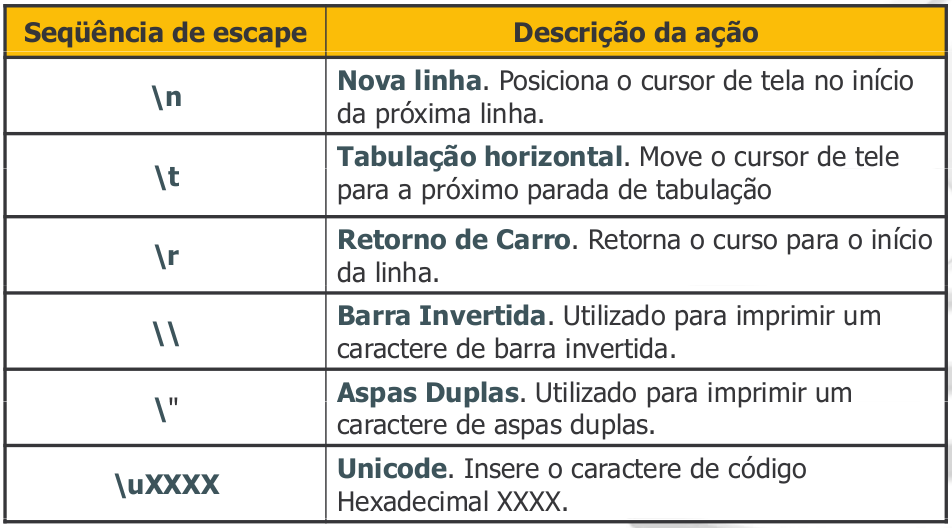
\includegraphics[height=0.6\paperheight]{caracteres_especiais.png} \\
 \end{center}
\end{frame}}
%----------------------------------------------------------------------------
\section{Tipos de dados}
\mode<presentation>{ \begin{frame}{Tipos de dados}
  Java é uma linguagem \textbf{fortemente tipada}, ou seja, só podemos usar uma 
variável depois de definirmos um tipo pra ela.\\

  \vspace{0.5cm}
   As variáveis podem ser de dois tipos:\\
   
   \begin{block}{Tipos de Dados Primitivos}
    \textit{São semelhantes as variáveis comuns em linguagens estruturadas,  
simplesmente armazenam um valor.}
   \end{block}
  \vspace{0.5cm}

   \begin{block}{Tipos de dados Construídos}
     \textit{São as classes construídas, que podem estar definidas no Java ou 
serem criadas pelo programador.}
   \end{block}
\end{frame}}
%----------------------------------------------------------------------------
\mode<presentation>{ \begin{frame}{Tipos de dados Primitivos}
\begin{center}
   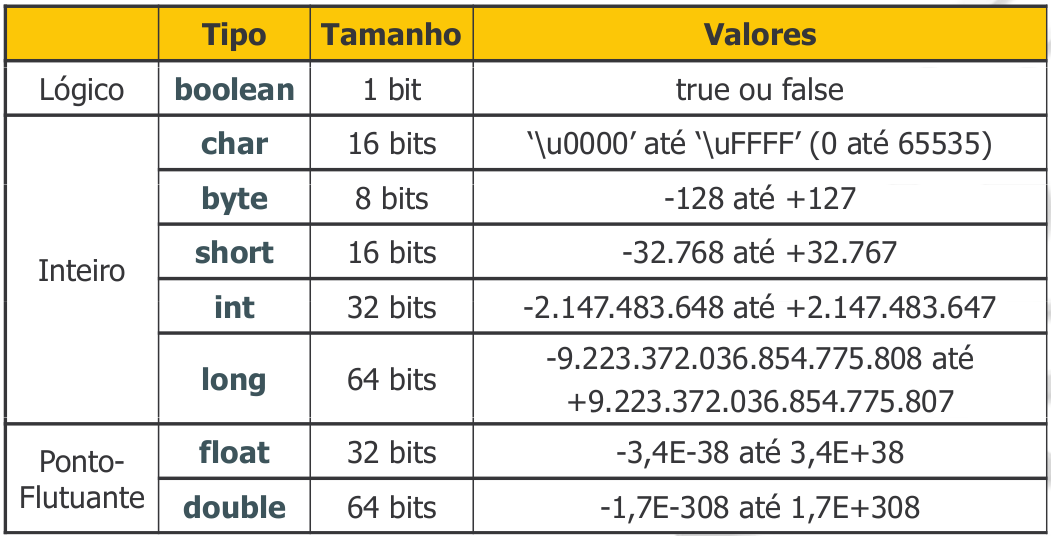
\includegraphics[height=0.5\paperheight]{primitivo.png} \\
 \end{center}
\end{frame}}
%----------------------------------------------------------------------------
\section{Identificadores}
\mode<presentation>{ \begin{frame}{Identificadores}
  \begin{itemize}
   \item São nomes de variáveis, métodos, classes, interfaces e pacotes, 
   definidos pelo usuário dentro do código
   \begin{itemize}
      \item Os nomes são \textbf{\textcolor{red}{case-sensitive}} 
(diferenciam maiúscula de minúscula).
     \item podem conter letras, números (\textbf{\textcolor{red}{0 a 
9}}), sublinhado (\textbf{\textcolor{red}{\_}}) e cifrão 
    (\textbf{\textcolor{red}{\$}}).
       \item NÃO podem começar com números.
       \item NÃO podem possuir espaços em branco
       \item NÃO podem ser iguais as palavras reservadas pela linguagem.
   \end{itemize}
    \item Extras
   \begin{itemize}
    \item Usar nomes sugestivos e seguir as recomendações da Oracle.
   \end{itemize}
  \end{itemize}
\end{frame}}
%----------------------------------------------------------------------------
\mode<presentation>{ \begin{frame}{Exemplo}
  \begin{block}{Identificadores válidos}
    \begin{columns}
    \begin{column}{0.5\textwidth}
      \begin{itemize}
	\item int \textbf{Idade};
	 \item int \textbf{idade};
	 \item String \textbf{nomeCliente};
	 \item int \textbf{\_A\$\_09};
      \end{itemize}
      \end{column}  
      \begin{column}{0.4\textwidth}
%       \vspace{0.2cm}
      \tiny{
	Idade e idade: 
      \textbf{\textcolor{red}{São variáveis diferentes, pois Java 
diferencia minúscula de maiúscula.}}\\
      }
    \end{column}
  \end{columns}
   \end{block}
    
    
    \begin{block}{Identificadores inválidos}
     \begin{itemize}
       \item int \textbf{9Numeros};  // iniciando com 
número
	 \item String \textbf{Nome Cliente}; // possui espaço em 
branco
	 \item public class \textbf{\%exemplo\%}; // 
possui caractere inválido
	 \item int \textbf{return}; // uso de palavra reservada
     \end{itemize}

    \end{block}
    
\end{frame}}
%----------------------------------------------------------------------------
\mode<presentation>{ \begin{frame}{Palavras Reservadas}
\begin{center}
   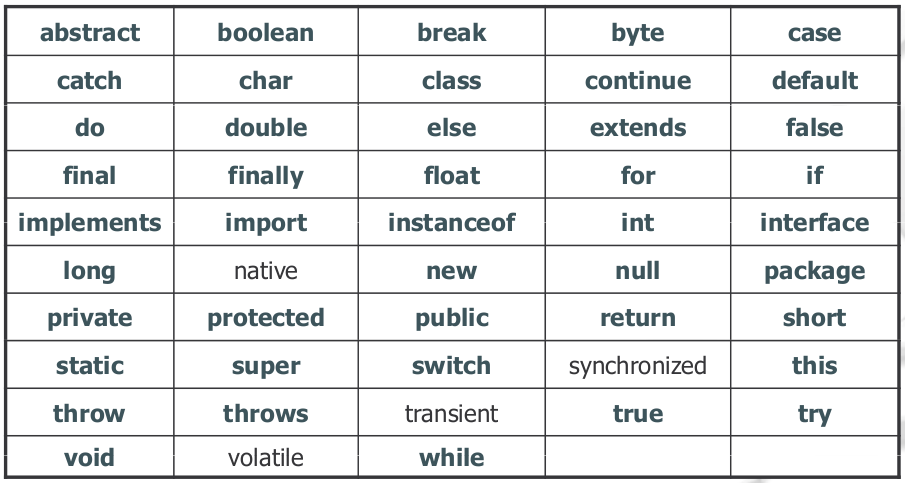
\includegraphics[height=0.6\paperheight]{reservada.png} \\
 \end{center}
\end{frame}}
%----------------------------------------------------------------
\mode<presentation>{ \begin{frame}{Padrão da linguagem}
  \begin{block}{Variáveis e métodos}
   \begin{itemize}
    \item Iniciam o nome com letra minúscula;
     \item Nomes compostos separar por meio de letras maiúsculas
     \item \textbf{Ex:} nomeDeVariavel, nomeDeMetodo.
   \end{itemize}
  \end{block}
\end{frame}}
%----------------------------------------------------------------
\mode<presentation>{ \begin{frame}{Padrão da linguagem}
  \begin{block}{Classes}
   \begin{itemize}
    \item Iniciam o nome com letra Maiúscula;
     \item Nomes compostos separar por meio de letras maiúsculas
     \item \textbf{Ex:} NomeDeClasse.
   \end{itemize}
  \end{block}
  \begin{block}{Constantes}
   \begin{itemize}
    \item Todas as letras Maiúsculas, separadas por (\_)
    \item Ex: TOTAL\_ALUNOS.
   \end{itemize}
  \end{block}
\end{frame}}
%----------------------------------------------------------------
\section{Operadores}
\mode<presentation>{ \begin{frame}{Operadores}
  \begin{itemize}
   \item (\textbf{=}) Copia o valor da variável da direita para a variável da 
esquerda. 
     \item int idade \textbf{=} 57;
     \item double salario \textbf{=} 1300.00, abono \textbf{=} 600.00;
  \end{itemize}

\end{frame}}
%----------------------------------------------------------------------------
\mode<presentation>{ \begin{frame}{Operadores aritméticos}
\begin{center}
   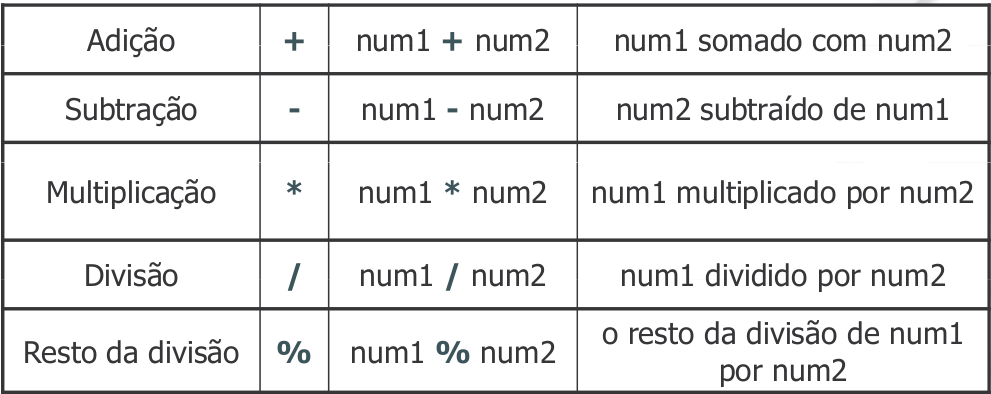
\includegraphics[height=0.4\paperheight]{aritimeticos.png} \\
 \end{center}
\end{frame}}
%----------------------------------------------------------------------------
\mode<presentation>{ \begin{frame}{Operadores relacionais}
  Avaliam uma expressão e retornam \textbf{\textcolor{red}{true}} ou 
\textbf{\textcolor{red}{false}};
\begin{center}
   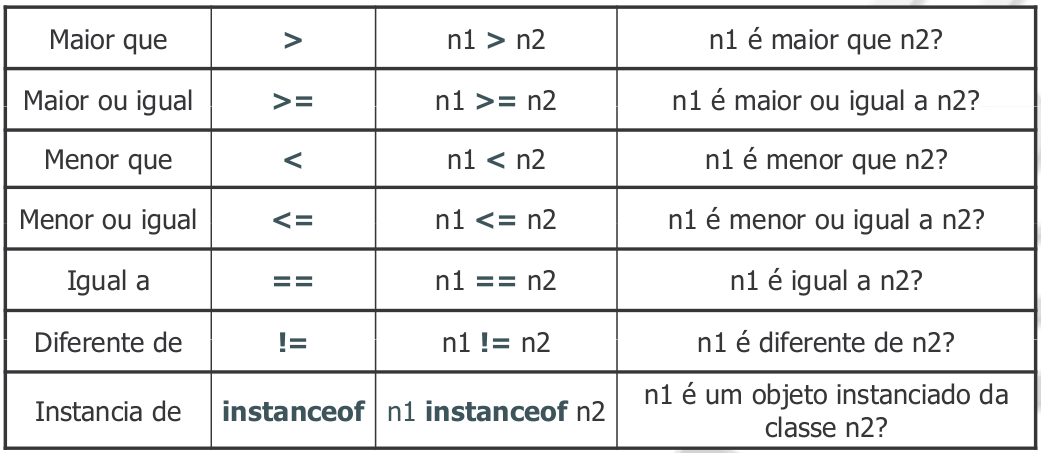
\includegraphics[height=0.5\paperheight]{relacionais.png} \\
 \end{center}
\end{frame}}
%----------------------------------------------------------------------------
\mode<presentation>{ \begin{frame}{Operadores lógicos}
  Avaliam uma expressão lógica e retornam \textbf{\textcolor{red}{true}} ou 
\textbf{\textcolor{red}{false}};
\begin{center}
   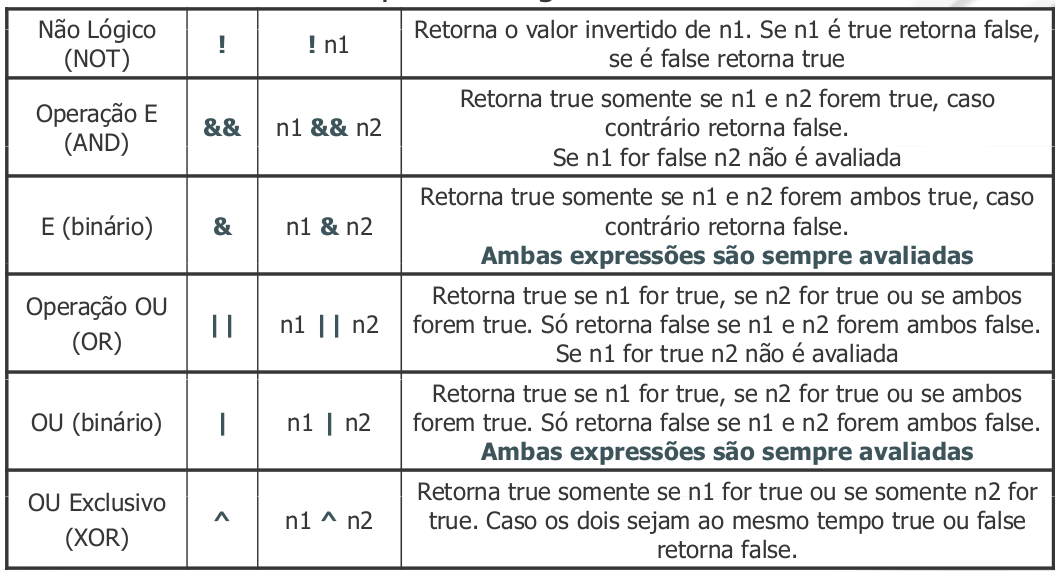
\includegraphics[height=0.55\paperheight]{logicos.png} \\
 \end{center}
\end{frame}}
%----------------------------------------------------------------------------
\mode<presentation>{ \begin{frame}{Operadores de atribuição composta}
\begin{center}
   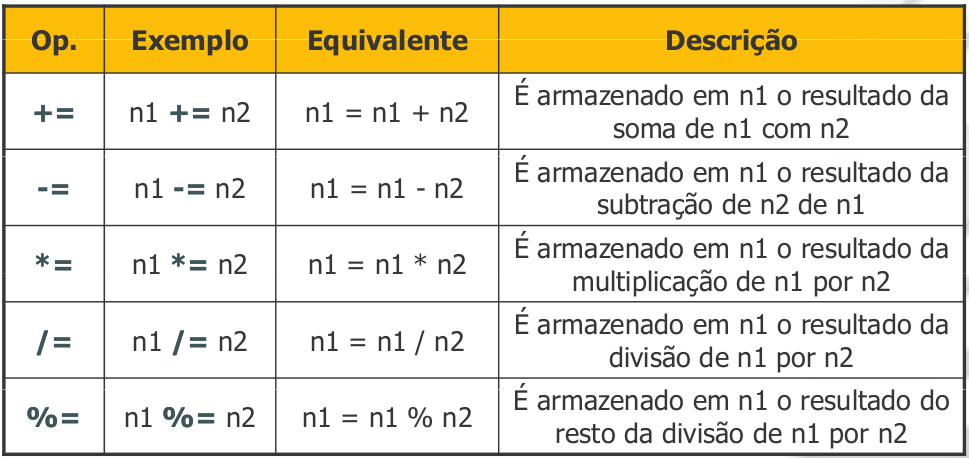
\includegraphics[height=0.55\paperheight]{atribuicao_composta.png} \\
 \end{center}
\end{frame}}
%----------------------------------------------------------------------------
\mode<presentation>{ \begin{frame}{Operadores de incremento e decremento}
\begin{center}
   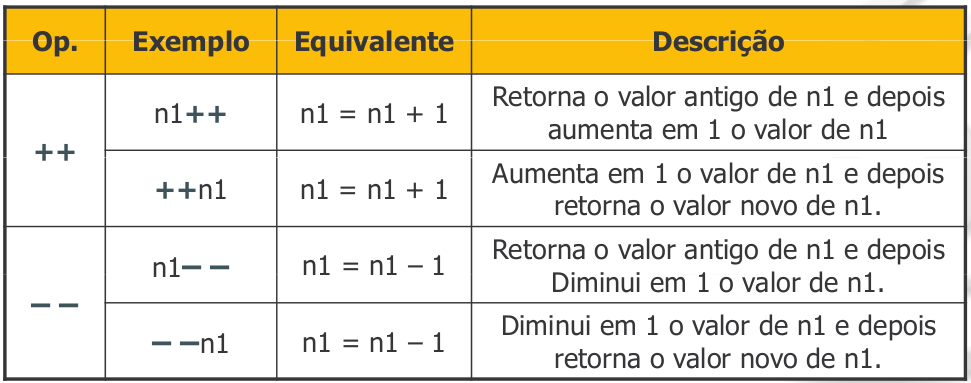
\includegraphics[height=0.45\paperheight]{incremento_dec.png} \\
 \end{center}
\end{frame}}
%----------------------------------------------------------------------------
\mode<presentation>{ \begin{frame}{Precedência de Operadores}
  Ordem na qual as operações serão executadas.
\begin{center}
   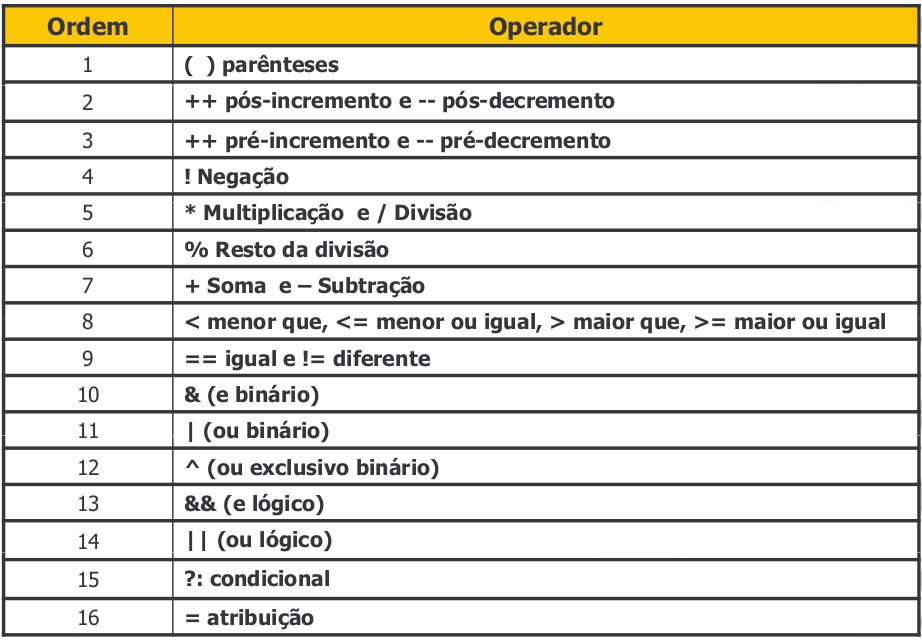
\includegraphics[height=0.65\paperheight]{precedencia.png} \\
 \end{center}
\end{frame}}

%-------------------------------------------------------------------------
\section{Estruturas de controle}
\subsection{Estruturas de seleção}
\mode<presentation>{ \begin{frame}{Estruturas de seleção - IF}
  A partir do teste de uma condição executa ou não um conjunto de instruções.
\begin{center}
   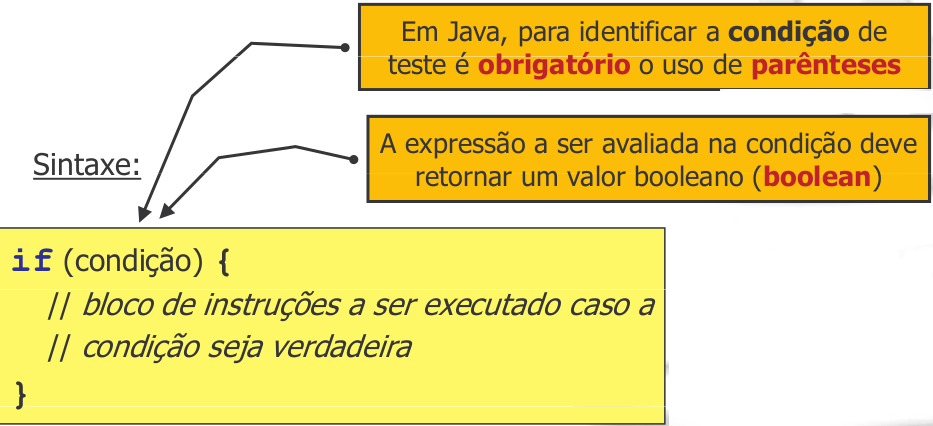
\includegraphics[height=0.5\paperheight]{if.png} \\
 \end{center}
\end{frame}}
%-------------------------------------------------------------------------
\mode<presentation>{ \begin{frame}{Estruturas de seleção - IF}
 \begin{center} 
\lstinputlisting[linerange={3-6}]{./cod/Aula3Exemplos.java}
  \end{center}
\begin{center}
   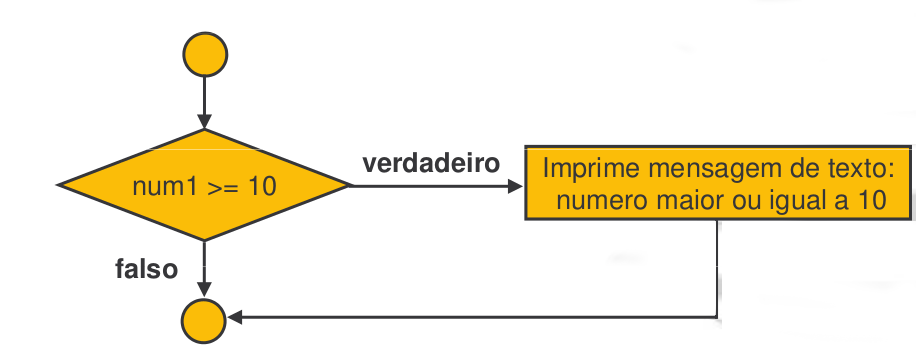
\includegraphics[height=0.3\paperheight]{if_fluxo.png} \\
 \end{center}
\end{frame}}
%----------------------------------------------------------------------
\mode<presentation>{ \begin{frame}{Estruturas de seleção - IF/ ELSE}
 \begin{center}  
  \lstinputlisting[linerange={3-8}]{./cod/Aula3Exemplos.java}
 \end{center}
\end{frame}}
%----------------------------------------------------------------------
\mode<presentation>{ \begin{frame}{Estruturas aninhadas}
 
\begin{center}
  \lstinputlisting[linerange={10-23}]{
./cod/Aula3Exemplos.java}
 \end{center}
\end{frame}}
%----------------------------------------------------------------------
\mode<presentation>{ \begin{frame}{Estruturas aninhadas}
 
\begin{center}
  \lstinputlisting[linerange={26-35}]{
./cod/Aula3Exemplos.java}
 \end{center}
\end{frame}}
%----------------------------------------------------------------------
\mode<presentation>{ \begin{frame}{Operador Ternário}
 teste lógico ? valorSeVerdadeiro : valorSeFalso
 \begin{center}
   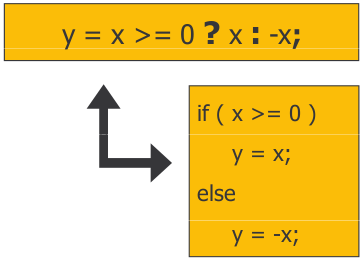
\includegraphics[height=0.3\paperheight]{ternario.png} \\
   Exemplo:\\
  \lstinputlisting[linerange={38-38}]{
./cod/Aula3Exemplos.java}
 \end{center}
\end{frame}}
%-------------------------------------------------------------------------
\mode<presentation>{ \begin{frame}{Estruturas de seleção - \textbf{Switch}}
  Chamada de \textbf{estrutura de seleção múltipla}, pois a partir da 
comparação de um valor passado com os outros valores definidos, seleciona um 
ponto do qual iniciará a execução de um conjunto de instruções.
 \begin{center} 
\lstinputlisting[linerange={40-48}]{./cod/Aula3Exemplos.java}
  \end{center}
\end{frame}}
%-------------------------------------------------------------------------
\mode<presentation>{ \begin{frame}{Estruturas de seleção - \textbf{Switch}}
 \begin{center}
   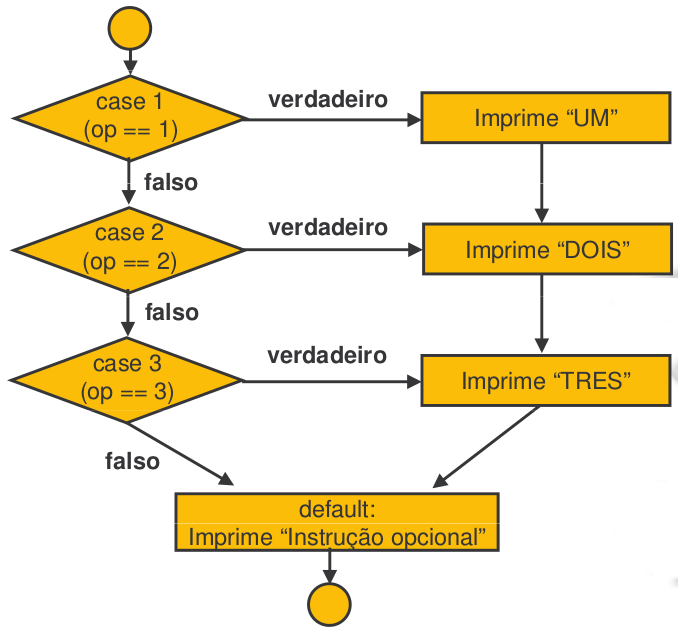
\includegraphics[height=0.6\paperheight]{switch.png} \\
  \end{center}
\end{frame}}
%-------------------------------------------------------------------------
\mode<presentation>{ \begin{frame}{Estruturas de seleção - \textbf{Switch}}
 \begin{center} 
\lstinputlisting[linerange={49-59}]{./cod/Aula3Exemplos.java}
  \end{center}
\end{frame}}
%----------------------------------------------------------------------
\section{Atividades}
\mode<presentation>{ \begin{frame}{Atividade}
  \textbf{1.} Faça um programa usando os operadores relacionais que escreva no 
console, seguinte saída:
  \begin{center}
   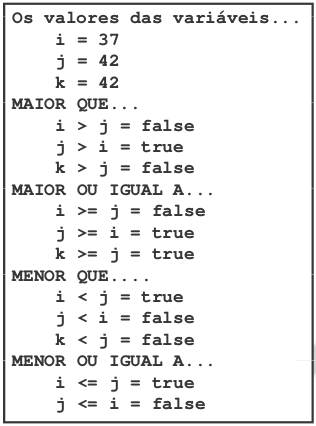
\includegraphics[height=0.6\paperheight]{atividade1_aula3.png} \\
  \end{center}
\end{frame}}
%----------------------------------------------------------------------
\mode<presentation>{ \begin{frame}{Atividade}
  \textbf{2.} Examine o código abaixo e determine qual o valor das variáveis i, 
j, x e y depois desses passos.
  \begin{center}
   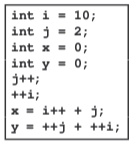
\includegraphics[height=0.4\paperheight]{atividade2_aula3.png} \\
  \end{center}
\end{frame}}
%----------------------------------------------------------------------
\mode<presentation>{ \begin{frame}{Atividade}
  \textbf{3.} Crie um programa que obtenha a média de 3 números. Considere o 
valor para os três números como sendo 10, 20 e 45. O resultado esperado do 
exercício é:
  \begin{center}
   número1 com o valor 10\\
   número2 com o valor 20\\
   número3 com o valor 45\\
   A média é 25
  \end{center}
    \textbf{4.} Dada as expressões abaixo, reescreva-as utilizando parênteses 
de acordo com a forma como elas são interpretadas pelo compilador.
  \begin{center}    
\lstinputlisting[linerange={60-62}]{./cod/Aula3Exemplos.java}
  \end{center}
\end{frame}}
%----------------------------------------------------------------------
\mode<presentation>{ \begin{frame}{Atividade}
  \textbf{5.} Faça um programa que leia três números reais representando os 
lados de um triângulo. Primeiramente verifique se os três lados formam um 
triângulo. Caso não formam imprima uma mensagem de erro para o usuário. Caso os 
lados formem um triângulo imprima qual é o tipo dele. Lembre-se que:
\begin{itemize}
    \item Só é triangulo se: \textit{um de seus lados deve ser maior que o valor absoluto (módulo) da diferença dos outros dois lados e menor que a soma dos outros dois lados}.
    \item \textbf{Equilátero:} todos os lados congruentes;
    \item \textbf{Isósceles:} dois lados congruentes;
    \item \textbf{Escaleno: }todos os lados com medidas distintas.
\end{itemize}
\end{frame}
}
%------------------------------
\section{Leitura recomendada}
\mode<presentation>{ \begin{frame}{Leitura complementar}
 Para mais informações sobre JAVA, leia:\\
	\begin{columns}
	\begin{column}{0.5\textwidth}
	 Capítulo 1 e 2:
	 \cite{deitel2017java}
	\end{column}
	\begin{column}{0.4\textwidth}
	
\includegraphics[height=0.6\paperheight]{fig/aula1/deitel2017java.png} 
	\end{column}
	\end{columns}
	%\textcolor{red}{DISPONÍVEL NA BIBLIOTECA VIRTUAL}
\end{frame}}

 %----------------------------------------------------------------------------
 
 \mode<presentation>{ \begin{frame}{Referências}%[allowframebreaks]
 \small
 \begin{center}
 	\bibliographystyle{apalike}
	 \bibliography{ref_aula_progI}
 \end{center}
 \end{frame}}

\begin{figure}[!ht] \fbox{\includeslide[width=\textwidth]{slide:z}} \end{figure}
Text for notes goes here. 
\begin{itemize}
  \item List 1. 
  \item List 2. 
\end{itemize}


%%%%%%%%%%%%%%%%%% END MATTER %%%%%%%%%%%%%%%%%%
\end{document}